
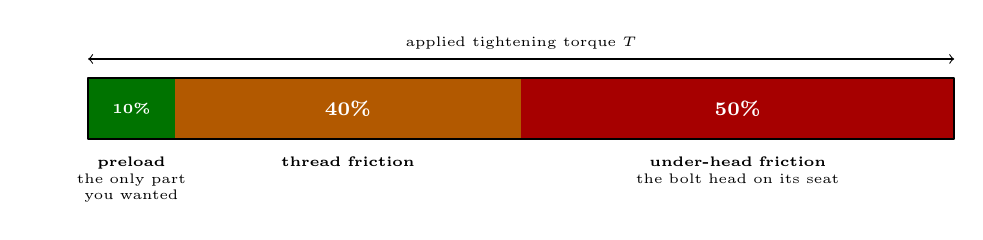
\begin{tikzpicture}[scale=1.0,font=\scriptsize,line join=round]
\def\W{11.0}
\fill[green!45!black] (0,0) rectangle (0.10*\W,0.78);
\fill[orange!70!black] (0.10*\W,0) rectangle (0.50*\W,0.78);
\fill[red!65!black] (0.50*\W,0) rectangle (\W,0.78);
\draw[thick] (0,0) rectangle (\W,0.78);
\node[white,font=\bfseries\tiny] at (0.05*\W,0.39) {10\%};
\node[white,font=\bfseries\scriptsize] at (0.30*\W,0.39) {40\%};
\node[white,font=\bfseries\scriptsize] at (0.75*\W,0.39) {50\%};
\node[anchor=north,align=center,font=\tiny,text width=2.4cm] at (0.05*\W,-0.10)
  {\textbf{preload}\\ the only part you wanted};
\node[anchor=north,align=center,font=\tiny,text width=3.0cm] at (0.30*\W,-0.10)
  {\textbf{thread friction}};
\node[anchor=north,align=center,font=\tiny,text width=3.2cm] at (0.75*\W,-0.10)
  {\textbf{under-head friction}\\ the bolt head on its seat};
\draw[<->] (0,1.02) -- (\W,1.02) node[midway,above,font=\tiny] {applied tightening torque $T$};
\end{tikzpicture}
